I denne delen blir probleminstanser, løsningsstrategier og løsninger evaluert. Denne delen blir avsluttet med å evaluere løsningene funnet i dette prosjektet opp mot løsningene funnet i artikkelen til Bård Henning Tvedt.

Generelle forutsetninger for probleminstansene er:
Med 10 lokasjoner vil vil det i snitt være 5-500 aktiviteter pr. lokasjon. Varmekapasitet er en gitt verdi på hver lokasjon. Det er å forvente at:
\begin{itemize}
\item jo flere aktiviteter, desto større blir effekten av varmekapasiteten på lokasjonen.
\item jo høyere aktivitet (større behov for kran), desto større begrensende effekt vil kranressursene få.
\end{itemize}

\subsection{Probleminstanser}
Probleminstansene har fra 50-5000 aktiviteter, mens antall lokasjoner og mannskaper i de genererte probleminstansene er henholdsvis 10 og 5.

Det ble først eksperimentert litt med mannskapets varme og lokasjoners varmekapsitet og i det første settet med probleminstanser var det overlapp mellom mannskapers varme og en lokasjons varmekapasitet. Dette førte til veldig få løsninger når varmebegrensningen ble tatt med. Det ble funnet løsninger på noen av probleminstansene under 100 aktiviteter, mens over 100 aktiviteter var det kun en løsning. Det er grunn til å tro dette var tilfeldig, ut i fra at varme og varmekapasitet blir tilfeldig plassert innenfor et gitt område. Erfaringene fra dette er kun tatt til etterretning og resultatene er ikke interessante her pga. få løsninger.

Probleminstansene hvor varme og varmekapasitet ikke er overlappende, ga flere løsninger og er brukt videre gjennom prosjektoppgaven.

\subsection{Løsningsstrategier}
Tabell \ref{tab:resultaterSum100s} viser et ganske klart bilde av de sterke og svake sidene til de to løsningsstrategiene som er brukt. LS1 løser alle probleminstanser, mens LS2 gir betydelig bedre makespan.

Ser vi samtidig på ressursskjemaene for $LS1\sharp1\sharp3$, figur \ref{fig:RessursWithoutAct50Loc10Crew5Crane2LS1}, og $LS2\sharp1\sharp3$, figur \ref{fig:ResourceAct50Crane2LS2_UtenVarme_100s}, for gitte tilfeller, ser vi følgende:
\begin{itemize}
\item $LS1\sharp1\sharp3$ har få aktiviteter mot enden av tidsaksen. Det er lengere makespan.
\item $LS2\sharp1\sharp3$ har jevnt med aktiviteter langs tidsaksen. Det er kortere makespan.
\end{itemize}
I henhold til tidligere skisserte forventninger har dette mest sannsynlig sin årsak i at LS1 produserer flere løsninger fordi kraner med sine begrensninger er på plass tidlig i søkeprosessen.
LS2 produserer bedre løsninger fordi det tildeles startverdier til aktiviteter uten å betrakte kranfordelingen så nøye. Men antallet løsninger blir gjerne redusert fordi søkeprosessen ikke klarer å komme ut av konfliktene som oppstår når man tildeler kran senere.

Modellene uten sikkerhetsbegrensinger ga identiske løsninger. Dette er muligens fordi når sikkerhetsbegrensning på kran fjernes fungerer LS1 og LS2 likt.

\subsection{Resultater}
I denne prosjektoppgaven er en eksisterende løsning utvidet med en ressurs kalt varmeressurs. For å evaluere resultatene fra den utvidete løsningen, evalueres den utvidete løsningen med 10 lokasjoner opp mot den opprinnelige løsningen med 25 lokasjoner. Hensikten med å sammenligne resultatene fra den opprinnelige løsningen med 25 lokasjoner og 10 lokasjoner er å analysere effekten av antall lokasjoner.

Evalueringen innebærer også å analysere effekten av varmebegrensningen, som er gjort ved å sammenligne resultatene med 10 lokasjoner med og uten varmebegrensning. Evalueringen av resultatene baserer seg på gjennomsnittsverdiene i tabell \ref{tab:resultaterSum100s} og \ref{tab:resultaterSum5s}.

\subsubsection{10 Lokasjoner}
Løsningene er i ganske god overensstemmelse med forventningene i kapitel \ref{sec:implprocess}. Med LS1 hvor kranfordelingen ble valgt først var gjennomsnittlig makespan dårligere enn med LS2.

\begin{figure}[!h]
\centering
\includegraphics[scale=0.3]{content/gfx/Act50Crane2AssignHeatResourceCrane}
\caption{Ressursoversikt på Act50Loc10Crew5Crane2 med varmebegrensning, LS1, $\sharp2\sharp3$}
\label{fig:RessursWithAct50Loc10Crew5Crane2LS1}
\end{figure}
\begin{figure}[!h]
\centering
\includegraphics[scale=0.3]{content/gfx/Act50Crane2WithoutResourceCrane}
\caption{Ressursoversikt på Act50Loc10Crew5Crane2 uten varmebegrensning, LS1, $\sharp1\sharp3$}
\label{fig:RessursWithoutAct50Loc10Crew5Crane2LS1}
\end{figure}
\begin{figure}[!h]
\centering
\includegraphics[scale=0.3]{content/gfx/Act50Crane3AssignHeatResourceCrew}
\caption{Ressursoversikt på Act50Loc10Crew5Crane3 med varmebegrensning, LS1 og $\sharp2\sharp3$}
\label{fig:RessursWithAct50Loc10Crew5Crane3LS1}
\end{figure}
\begin{figure}[!h]
\centering
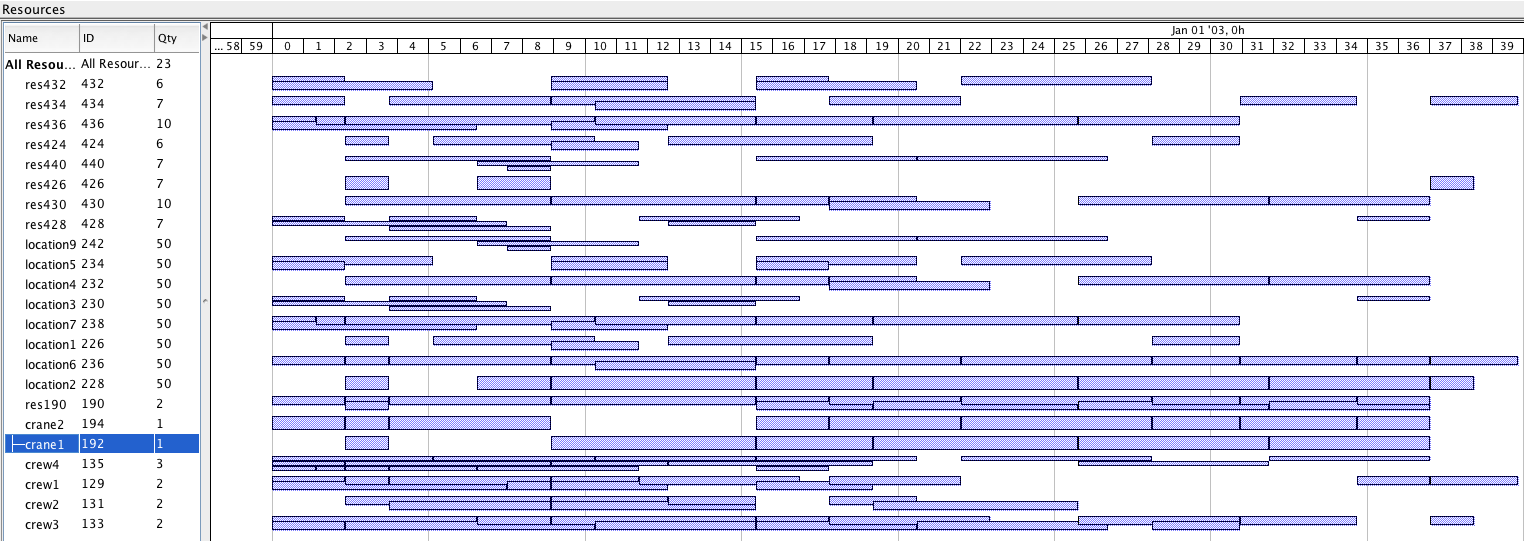
\includegraphics[scale=0.3]{content/gfx/Act50Crane2LS2WithHeat}
\caption{Ressursoversikt på Act50Loc10Crew5Crane2 med varmebegrensning, LS2 og $\sharp2\sharp3$}
\label{fig:RessursWithAct50Loc10Crew5Crane2LS2}
\end{figure}
Figur \ref{fig:RessursWithAct50Loc10Crew5Crane2LS1} og \ref{fig:RessursWithAct50Loc10Crew5Crane3LS1} er ressursdiagrammer med varmebegrensing. Til venstre i disse bildene er ressursene listet opp. De 8 øverst i denne listen er varmeressursene. Deretter følger lokasjons- og kranressursene, hvor det også er 8 lokasjonsressurser. I og med at varmeressursen er knyttet til lokasjon, er det samme antall varmeressurser som lokasjonsressurser. I og med at varmebegrensningen er knyttet til en aktivitet og lokasjonene er knyttet til en aktivitet, er det aktiviteter i disse figurene som har samme varighet under varmebegrensningen og på lokasjonsressursen. Dette er tydelig til høyre på figurene hvor det ikke er så mange aktiviteter.

Figur \ref{fig:RessursWithoutAct50Loc10Crew5Crane2LS1} er en gitt situasjon uten varmebegrensning og figur \ref{fig:RessursWithAct50Loc10Crew5Crane2LS1} er den samme med varmebegrensning. Begge figurene har lokasjon 2 fullt utnyttet. Kran 1 er på lokasjonen og er den reelle begrensningen. Innføring av varmebegrensningen gir i dette tilfellet med kran som begrensning lite utslag i henhold til tabell \ref{tab:resultaterSum100s} (liten økning i makespan). Generelt er det forventet en økning i makespan når varmebegrensing innføres. Denne økningen antas ikke i sin helhet å kun komme fra varmebegrensningen, men sannsynligvis også være et resultat at det blir vanskeligere å løse problemet.

Figur \ref{fig:RessursWithAct50Loc10Crew5Crane3LS1} kontra figur \ref{fig:RessursWithoutAct50Loc10Crew5Crane2LS1} er en gitt situasjon og økning fra to til tre kraner. Det er samme betrakning rundt utnyttelse, men i figur \ref{fig:RessursWithAct50Loc10Crew5Crane3LS1} endres dette. Her er det nå mannskap som over tid bruker hele kapasiteten.

\begin{equation}
c_{load}(Crane_{k}) = \sum_{c_{Crane}(Act_{i})=Crane_{k}} c_{dur}(Act_{i})
\label{eq:kranstyrke}
\end{equation}
Ved å sammenligne om verdier fra (\ref{eq:kranstyrke}) er mindre eller større enn (\ref{eq:mannskapsstyrke}), gir det et uttrykk for hvor sterk eller svak kranressursen er. Hvis (\ref{eq:kranstyrke}) er mindre vil det si at kranressursen er svak. Ut ifra dette er det en signifikant forskjell på to og tre kraner med LS1. Ved to kraner er kranressursen veldig sterk på kran 1, mens kranressursen ikke er fullt så sterke med tre kraner. Figur \ref{fig:RessursWithAct50Loc10Crew5Crane2LS1} viser den skjeve fordelingen mellom kran 1 og kran 2. Denne figuren viser tydelig at kran 1 er ganske godt utnyttet, mens kran 2 er mindre utnyttet. De tre aktivitetene som er helt til høyre i figur \ref{fig:RessursWithAct50Loc10Crew5Crane2LS1} krever alle kran og er tildelt kran 1. Med LS2 er det en jevnere kranfordeling som også vises i figur \ref{fig:RessursWithAct50Loc10Crew5Crane2LS2}. Med en jevnere utnyttelse av kranene som i LS2 vil også makespan kunne bli bedre. Fra resultatene og målingene gjort med (\ref{eq:kranstyrke}) opp mot (\ref{eq:mannskapsstyrke}) og ved å studere figur \ref{fig:RessursWithAct50Loc10Crew5Crane2LS1} og \ref{fig:RessursWithAct50Loc10Crew5Crane2LS2}, virker det som å tildele kraner først i søkemålet i Solver så klarer man ikke å utnytte alle kranressursene som er tilgjengelig. Men når starttidene til aktivitetene blir tildelt først virker det som tildelingen av kraner klarer å utnytte kranressursene som er tilgjengelige på en bedre måte. En mulig forklaring kan være at ved å tildele kraner først, så vil søkerommet fortsatt være såpass stort at Solver ikke finner andre mulige kraner. Det er mulig at søkerommet ved å tildele starttider til aktiviteter først vil gjøre søkerommet mindre, så det å tildele kraner etter tildeling av starttider gjør Solver i stand til å finne beste mulige kranen til aktiviteter som krever det.

Det ble tidligere fremsatt forventninger til varmebegrensningen og kraners effekt på løsningene når antall aktiviteter øker. Dette ser i all hovedsak ut til å stemme ut ifra resultatene som fremkommer i tabell \ref{tab:resultaterSum100s} og \ref{tab:resultaterSum5s}. At det er noen unntak, kan sannsynligvis forklares ved lav løsningsprosent, slik at optimale løsninger ikke kan etableres.

Tiden det tar å løse probleminstansene er også veldig lik uten noe spesielt mønster både med og uten varmebegrensning. Det er derfor litt bedre løsninger uten varmebegrensning.

Ved å ta utgangspunkt i LS2 uten varmebegrensing og uten sikkerhetsbegrensning på kran fra tabell \ref{tab:resultaterSum100s} er makespan totalt sett 1.0\% over teoretisk nedregrense med tidsgrense på 100 sekunder. Det er også løsninger på alle probleminstanser. Denne løsningen er veldig lite begrenset, da det ikke er noen grense for hvor mange mannskaper som kan være på en lokasjon og heller ingen begrensning på gjennomføring av aktiviteter ved kranbruk. Når sikkerhetsbegrensningene blir lagt til øker makespan med 13.2\% og det er ikke løsninger på mer enn 36.88\% av probleminstansene. Dette virker fornuftig med tanke på at sikkerhetsbegrensningene vil opprette sikkerhetssoner som vil stenge lokasjonen til kranen og stenger lokasjonen aktiviteten som bruker kranen blir utført på. Ytterligere øker makespan med 9\% og det blir funnet løsninger på 40\% av probleminstansene da varmebegrensningen blir lagt til. Dette viser at det kan være en tendens at innføringen av varmebegrensningen bidrar til at Scheduler finner flere løsninger. Ved å se på tabell \ref{tab:resultaterSum5s} kan det se ut som tendensen også er gjeldene med en søketid på 5 sekunder. Her er løsningsprosentene for henholdsvis LS2$\sharp 1\sharp3$ og LS2$\sharp 2\sharp3$ 36\% og 37\%. Når varmebegrensningen blir lagt til, begrenses antall mannskaper som kan jobbe på lokasjonene samtidig. Det kan se ut som Scheduler sliter med sikkerhetsbegrensningene på kran.

\subsubsection{10 lokasjoner mot 25 lokasjoner}
For å sammenligne løsningene i denne prosjektoppgaven med 10 lokasjoner, mot løsningene til \bht med 25 lokasjoner, er tabell \ref{tab:resultaterSumTvedt} hentet fra \cite{tvedtbezem}. Det benyttes henholdsvis $LS2\sharp1\sharp3$ og Inferred i sammenlikningen.
\begin{table}[!h]
\caption{Relativ optimalitets indeks $w_{rq}$ for de forskjellige modellene}
\begin{center}
\begin{tabular}{ | c | c | c | c | c | c | c | c | c | c | c | }
\hline
\textbf{Modell} & \multicolumn{4}{|c|}{\textbf{2 kraner}} & \multicolumn{4}{|c|}{\textbf{3 kraner}} & \multicolumn{2}{|c|}{\textbf{Alle}} \\ \hline
$\sharp Act(\sharp P)$ & \multicolumn{2}{|c|}{$< 100 (25)$} & \multicolumn{2}{|c|}{$> 100 (23)$} & \multicolumn{2}{|c|}{$< 100 (28)$} & \multicolumn{2}{|c|}{$> 100 (23)$} & \multicolumn{2}{|c|}{(99)} \\ 
\hline
Modell & $w_{rq}$ & $\%^{(2)}$ & $w_{rq}$ & $\%^{(2)}$  & $w_{rq}$ & $\%^{(2)}$ & $w_{rq}$ & $\%^{(2)}$ & $w_{rq}$ & $\%^{(2)}$ \\ \hline
Greedy & 1.311 & 100 & 1.524 & 100 & 1.276 & 100 & 1.393 & 100 & 1.370 & 100 \\
Inferred & 1.068 & 100 & 1.063 & 35 & 1.017 & 32 & 1.000 & 4 & 1.055 & 43 \\
Under$^{(1)}$ & 1.032 & 100 & 1.014 & 100 & 1.015 & 100 & 1.002 & 96 & 1.016 & 99 \\
Over$\sharp 1$ & 1.143 & 100 & 1.076 & 100 & 1.176 & 100 & 1.037 & 91 & 1.114 & 98 \\
Over$\sharp 2$ & 1.104 & 100 & 1.047 & 96 & 1.068 & 96 & 1.005 & 65 & 1.063 & 90 \\
\hline
\multicolumn{11}{l}{\begin{minipage}{6in}$^{(1)}$ Denne modellen garanterer ikke gyldige løsninger.
$^{(2)}$ prosentandel løste instanser \end{minipage}}
\end{tabular}
\end{center}
\label{tab:resultaterSumTvedt}
\end{table}
Det er stort samsvar mellom både makespan og løsningsgrad. Makespan er bra og varierer lite. Løsningsgrad reduseres svært mye med mange aktiviteter, både for to og tre kraner. I begge modellene tildeles tid til aktiviteter før kranressurser. Som tidligere også beskrevet om LS2 antas tendensen å skyldes at kranressurser skal tildeles i et økende antall allerede disponerte aktiviteter. I Inferred modellen i tabell \ref{tab:resultaterSumTvedt} er makespan litt bedre enn i LS2$\sharp1\sharp3$ i tabell \ref{tab:resultaterSum100s}. Dette kan muligens forklares med reduksjonen av antall lokasjoner fra 25 i tabell \ref{tab:resultaterSumTvedt} til 10 i tabell \ref{tab:resultaterSum100s}. Det blir brukt samme antall kraner, 2 og 3, som med sikkerhetssonene aktivert vil låse en mye større andel av lokasjonene i løsningene med 10 lokasjoner enn løsningene med 25 lokasjoner. Med henholdsvis 2 kraner i bruk og aktiviteter som ikke utføres på samme lokasjon som kranen befinner seg, vil det da med sikkerhetssoner bli låst 4 lokasjoner. I løsningene med 10 lokasjoner vil da 40\% av lokasjonene være låst, mens med 25 lokasjoner vil bare 16\% av lokasjonene være låst pga. sikkerhetssonene.